\begin{center}
	\section{Eluci\'on y filtrado}
\end{center}

\noindent
\justify

La etapa de \textit{eluci\'on y filtrado} cumple el objetivo de obtener la mezcla l\'iquida homog\'enea solvente - extracto (FL). El material pulverizado $\left(m_p \right)$ se mezcla con un solvente, cuya polaridad permite aislar el extracto de la matriz s\'olida. El proceso posterior consiste en la separaci\'on de esta mezcla. 

\subsection{Dise\~no conceptual}

\noindent
\justify

De acuerdo a lo planteado en el primer informe de la Etapa III, el dise\~no conceptual de la planta de tratamiento, que se puede apreciar en la Figura \ref{trat}, consiste de una separaci\'on en dos etapas; en donde cada una de ellas emplea el mismo principio de separaci\'on: \textbf{diferencia de densidades}. El agente dispersante tiende a aglomerarse en el fondo del recipiente por ser el material de mayor densidad. El material vegetal, de menor densidad, tender\'a a flotar sobre la superficie superior de la planta; para evitar su paso sobre los decantadores, se dise\~naron con una superficie met\'alica externa de mayor altura que la boquilla de cada decantador. Esta boquilla cumple la funci\'on de separar los s\'olidos menos densos. Al final del tratamiento, se emplear\'a un filtro de papel, con f\'acil remoci\'on, para evitar el paso de s\'olidos residuales, obteniendo as\'i la mezcla \textit{solvente - extracto}.

\begin{figure}[h!]
\centering
\begin{minipage}[b]{0.48\textwidth}
	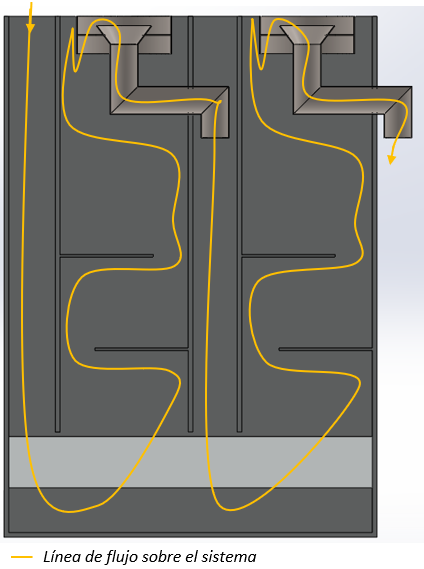
\includegraphics[width=\textwidth]{Images/Elution/flujo.PNG}
\end{minipage}
\hfill
\begin{minipage}[b]{0.48\textwidth}
	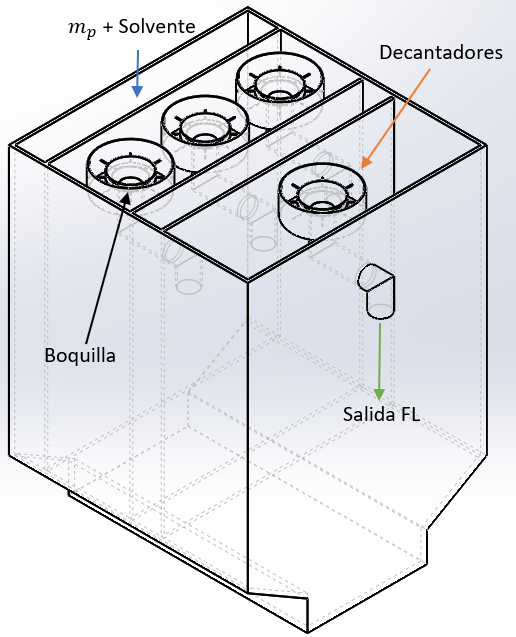
\includegraphics[width=\textwidth]{Images/Elution/filtrado2.PNG}
\end{minipage}
\caption{Planta de tratamiento.}
\label{trat}

\end{figure}


\newpage

\noindent
\justify

El espacio ocupado por la planta se puede apreciar en la Figura \ref{tratplano}.

\begin{figure}[h!]
	\centering
	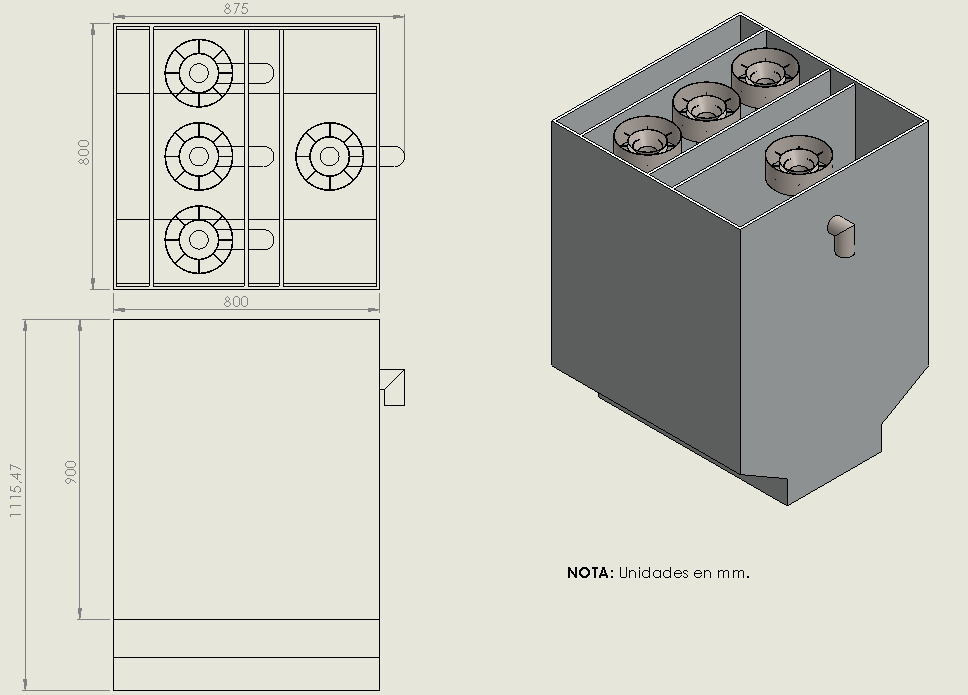
\includegraphics[width=\textwidth]{Images/Elution/plano_planta.jpeg}
	\caption{Distribuci\'on de espacio de la planta de tratamiento.}
	\label{tratplano}
\end{figure}

\subsection{Dise\~no funcional}

\noindent
\justify

Esta etapa tiene como objetivo proponer las variables operacionales del sistema, entre ellas: flujo m\'asico de entrada, temperatura inicial, posicionamiento de bafles y decantadores, entre otros; empleando metodolog\'ias de c\'alculo te\'orico propuestas en libros y art\'iculos de investigaci\'on a trav\'es de los siguientes datos de entrada: concentraci\'on inicial de soluto, tama\~no de part\'icula, propiedades termodin\'amicas del solvente, \'area de entrada y de salida del sistema.

\noindent
\justify

Una vez obtenidos estos resultados preliminares, se procede a desarrollar el modelo CFD del sistema empleando Python, Yade y OpenFOAM para realizar la verificaci\'on num\'erica del dise\~no y proponer mejoras que permitan obtener un resultado final \'optimo: mezcla homog\'enea \textit{solvente - extracto} con la menor concentraci\'on de part\'iculas posible.

\newpage

\subsection{Validaci\'on del dise\~no}

\noindent
\justify

Para validar tanto el dise\~no funcional como el modelo CFD planteado, se desarrollar\'an pruebas experimentales a una planta de tratamiento de aguas residuales operativa ubicada en la finca Los \'Angeles, P\'aramo, Santander; en donde se evaluar\'an los siguientes datos en, por lo menos, tres puntos clave del sistema (inicial, medio y final):

\begin{itemize}
	\item Velocidad de flujo.
	\item Presi\'on.
	\item Concentraci\'on de part\'iculas.
\end{itemize}

\noindent
\justify

Con estos resultados experimentales en cada punto de inter\'es, se podr\'a cuantificar el error medio del modelo CFD permitiendo desarrollar mejoras en la metodolog\'ia de c\'alculo.

\subsection{Dise\~no estructural}

\noindent
\justify

El dise\~no estructural consiste en definir diferentes par\'ametros, entre ellos: espesores de l\'amina, tipo de soldadura y de anclajes que garanticen tanto la integridad f\'isica del sistema como la del personal a cargo del mismo. Para ello, se emplear\'an metodolog\'ias de c\'alculo expuestas en libros de dise\~no mec\'anico, normativas nacionales e internacionales de dise\~no estructural y a trav\'es de simulaciones num\'ericas que empleen el m\'etodo de elementos finitos (FEM).